\documentclass{standalone}
\usepackage{tikz}
\usepackage{amsmath}
\usepackage{amssymb}

\begin{document}

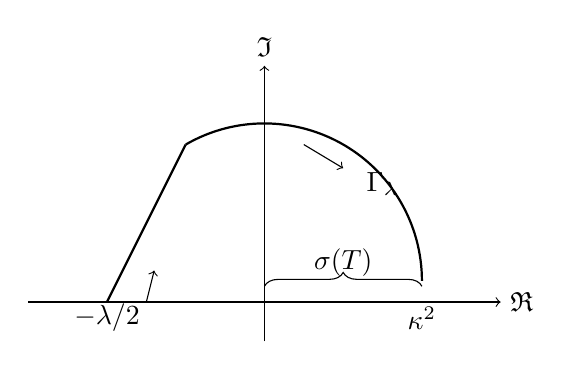
\begin{tikzpicture}
    % Axes
    \draw[->] (-3,0) -- (3,0) node[right] {$\mathfrak{R}$};
    \draw[->] (0,-0.5) -- (0,3) node[above] {$\mathfrak{I}$};

    % Contour
    \draw[thick] (0,0) -- (-2,0);
    \draw[thick] (-2,0) -- (-1,2);
    \draw[thick] (-1,2) arc[start angle=120, end angle=0, radius=2];

    % Dashed line and brackets
    \draw[dashed] (0,0) -- (2,0);
    \draw[decorate,decoration={brace,amplitude=5pt}] (0,0.2) -- (2,0.2) node[midway, above] {$\sigma(T)$};

    % Labels
    \node at (2,-0.2) {$\kappa^2$};
    \node at (-2,-0.2) {$-\lambda/2$};
    \node at (1.5,1.5) {$\Gamma_\lambda$};

    % Arrows on contour
    \draw[->] (-1.5,0) -- (-1.4,0.4);
    \draw[->] (0.5,2) -- (1,1.7);

\end{tikzpicture}

\end{document}